%\documentclass[12pt]{report}
%
%% some macros
%% Here, you can define your own macros. Some examples are given below.

\newcommand{\R}[0]{\mathds{R}} % real numbers
\newcommand{\Z}[0]{\mathds{Z}} % integers
\newcommand{\N}[0]{\mathds{N}} % natural numbers
\newcommand{\C}[0]{\mathds{C}} % complex numbers
\newcommand{\bm}[1]{{\boldsymbol{{#1}}}} % vector
\newcommand{\mat}[1]{{\boldsymbol{{#1}}}} % matrix

\newcommand{\E}[1]{\mathbb{E}_{#1}} % Expectation
\newcommand{\Pd}[1]{\mathbb{P}_{#1}} % Probability Distribution

%%%%%%%%%%%%%%%%%%%%%%%%%%%%%%%%%%%%%%%%%%
% University Assignment Title Page 
% LaTeX Template
% Version 1.0 (27/12/12)
%
% This template has been downloaded from:
%%%%%%%%%%%%%%%%%%%%%%%%%%%%%%%%%%%%%%%%%
%----------------------------------------------------------------------------------------
%	PACKAGES AND OTHER DOCUMENT CONFIGURATIONS
%----------------------------------------------------------------------------------------

\usepackage[nottoc,notlot,notlof]{tocbibind}
\usepackage[T1]{fontenc}
%\usepackage{hyperref}
\usepackage{indentfirst}
\usepackage{amsmath}
\usepackage{amssymb}
\usepackage{graphicx}
\usepackage{subcaption}
\usepackage{geometry}
 \geometry
 {
     a4paper,
     left=25mm,
     right=25mm,
     top=30mm,
     bottom=30mm,
 }

% \usepackage[a4paper,hmargin=2.8cm,vmargin=2.0cm,includeheadfoot]{geometry}
\usepackage{textpos}
\usepackage{natbib} % for bibliography
%\usepackage{tabularx,longtable,multirow,subfigure,caption}
\usepackage{fncylab} %formatting of labels
\usepackage{fancyhdr} % page layout
\usepackage{url} % URLs
\usepackage[english]{babel}
%\usepackage{dsfont}
\usepackage{epstopdf}
\usepackage{backref} % needed for citations
\usepackage{array}
\usepackage{latexsym}
\usepackage[pdftex,pagebackref,hypertexnames=false,colorlinks]{hyperref} % provide links in pdf
 
\hypersetup{pdftitle={},
  pdfsubject={}, 
  pdfauthor={},
  pdfkeywords={}, 
  pdfstartview=FitH,
  pdfpagemode={UseOutlines},% None, FullScreen, UseOutlines
  bookmarksnumbered=true, bookmarksopen=true, colorlinks,
    citecolor=black,%
    filecolor=black,%
    linkcolor=black,%
    urlcolor=black}
 
\usepackage[all]{hypcap}
\frenchspacing

\DeclareMathOperator{\tr}{tr}
%
%\begin{document}

\chapter{Deep Learning Background}
TODO add intro

\section{Convolutional Neural Networks}
Convolutional Neural Networks (CNNs) are a Machine Learning model architecture which uses a filter, or kernel, convolved over the input to extract features relevant to the given kernel from a small area of the input.
Multiple kernels are used at each layer of the model to extract multiple features, known as feature maps, from a given input image.
The CNN architecture is often paired with a downsampling layer to reduce the number of parameters in the model and prevent the model from growing too deep and becoming difficult to train due to vanishing gradients.
An activation function is applied to the output feature map from each convolutional layer to add non-linearities to the model. 

\subsection{Convolutional Layers}
Each convolutional layer is made up of a number of learnable kernels which are applied the the entire input image by sliding the kernels across the width and height of the image taking the dot product of the kernel and the current receptive field of the kernel for all channels of the input image, this is demonstrated in Figure \ref{fig:Conv_Layer}.
Each kernel is able to capture spatially relevant information about the current receptive field and pass this to the subsequent layers of the model.
During training these kernels are optimised to capture the most useful information for the task at hand.
The number of kernels used at each layer determines the number of feature maps produced, each of which are stacked as channels.
As each kernel is applied to the whole input image, the same learned parameters for each kernel are applied to the whole image, with each kernel extracting specific information.

\begin{figure}[h]
    \centering
        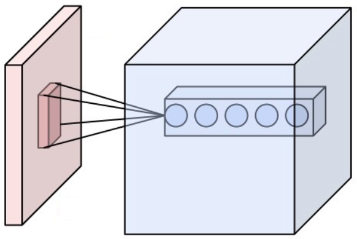
\includegraphics[width=0.5\textwidth]{figures/conv_layer.png}
    \caption{Convolutional Layer}\label{fig:Conv_Layer}
\end{figure}

\subsection{Layer Output Sizes}
An issue with convolutional layers is that the output image in slightly smaller than the input image as the kernel cannot be applied over the edge of the image.
For a given kernel size, the output image size can be calculated with equation (\ref{eq:conv_output}), where $H_{in}$ and $H_{out}$ represent in input and output sizes along one dimension, $k$ represents the size of the kernel along that dimension, $p$ is the padding applied to the input image and $s$ is the stride at which the kernel is applied to the image.

\begin{equation} \label{eq:conv_output}
    H_{out} = \frac{H_{in} + 2p - k}{s} + 1
\end{equation}

Padding can be applied to the image to increase the size of the input such that the output image is of the same size.
Commonly zero padding is applied, such that the image in padded with zeros around its border.

\subsubsection{Reducing Layer Output Size}
In order to prevent the models from becoming too deep and to limit the number of trainable parameters in a model, it is desirable to reduce the output feature map size.
To achieve this, pooling layers are commonly used, commonly either Max Pooling or Average Pooling.

\section{Activation Functions}
In order to add non-linearities to the model, activation functions are applied after each layer of models.
This non-linearity enables complex high order functions to be approximated by the network.

\subsection{Sigmoid}
The sigmoid function, expressed by equation (\ref{eq:sigmoid}) 

\begin{equation}\label{eq:sigmoid}
    \sigma(x) = \frac{1}{1 + e^{-x}}
\end{equation}

\subsection{Tanh}
\subsection{ReLU}

\section{Optimisation Algorithms}
\subsection{Stochastic Gradient Descent}
\subsection{Adam}
\subsection{RMSprop}

\section{Loss Functions}
\subsection{Negative Log Likelihood}
\subsection{Mean Squared Error?}

\section{Generative Adversarial Networks}

A recent development in generating synthetic data samples is the use of generative adversarial networks \cite{Goodfellow2014}.
The concept behind generative adversarial networks (GANs) is two have two machine learning models; a generator and a discriminator.
The task of the generator is to produce samples from an unknown high order probability distribution which correctly resemble samples from the distribution defined by training data.
The generator achieves this by transforming a random sample from a known probability distribution, such as a Gaussian distribution as used in \cite{Goodfellow2014}, to a sample from the unknown distribution.
This is achieved by finding the function which maps between the two distributions.
The discriminator however, attempts to correctly learn to discriminate between the real and the generated samples.

The original loss function (\ref{eq:gans_loss}) proposed by Ian Goodfellow forms a min-max game, where the loss of the generator is attempting to be minimised by having the discriminator label all the generated samples as real.
While the loss of the discriminator is maximised by correctly classifying real and fake samples.
Here $\bm{x}$ represent the real data samples from an unknown probability distribution $p_{data}$ and $\bm{z}$ represents a random noise sample from a known distribution.
The two networks are trained in an alternating fashion until the discriminator achieves an accuracy of 50\% on real and generated samples, effectively making binary guesses between the two.

\begin{equation} \label{eq:gans_loss}
    \min_{G} \max_{D} V(G, D) = \E{\bm{x} \sim p_{data}(\bm{x})} [\log D(\bm{x})]
                              + \E{\bm{z} \sim p_{z}(\bm{z})} [\log (1 - D(G(\bm{z})))]
\end{equation}
\quad

GANs however, are difficult to train for two main reasons.
Firstly, the equation (\ref{eq:gans_loss}) is challenging as it provides small gradients while generated samples are poor as discussed in \cite{Goodfellow2014}, making training difficult.
Progress in developing new loss functions is discussed in section \ref{Stability_to_GANs}
Secondly, early networks must also be balanced with a similar model capacity to prevent one from getting too much better than the other, preventing the other from improving.
Various architectural changes have improved this issue \cite{Radford2016, Zhang2018}, although it seems to be closely tied to the loss function being used \cite{Gulrajani2017}.

\subsection{Stability Improvements of GANs Networks} \label{Stability_to_GANs}
There have been a large number of papers presenting new techniques with differing levels of success and training stability, a small handful of key papers which provided large advances in the generative adversarial training model shall be discussed here.
A primary research focus around GANs has been in finding new loss functions on which to train the model to improve stability and performance.
The original loss function proposed in the original paper \cite{Goodfellow2014} identifies an issue with equation (\ref{eq:gans_loss}) in that the gradient back propagated to the generator when the generated samples are poor, is very low as shown in figure \ref{fig:Goodfellow_plot}.

\begin{figure}[h]
    \centering
        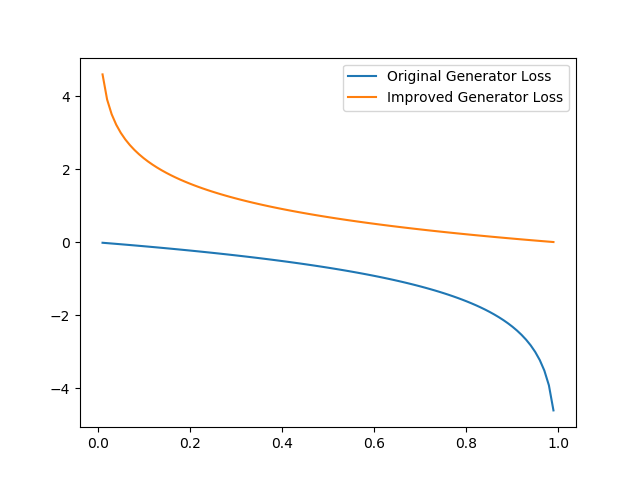
\includegraphics[width=0.8\textwidth]{figures/goodfellow_gen_losses.png}
    \caption{Goodfellow's Generator Loss Plots \cite{Goodfellow2014}}\label{fig:Goodfellow_plot}
\end{figure}
\quad

This in turn makes it very challenging to improve the performance of the generator.
The suggested improvement made in \cite{Goodfellow2014} is rather than to maximise the the number of generated samples which the discriminator incorrectly classifies, but to minimise the number of generator samples the discriminator correctly classifies, described in equation (\ref{eq:gans_loss2}).
Figure \ref{fig:Goodfellow_plot} shows how this results in the gradient propagated back to the generator is far larger when the generated samples are poor.

\begin{equation} \label{eq:gans_loss2}
    \min_{G} \max_{D} V(G, D) = \E{\bm{x} \sim p_{data}(\bm{x})} [\log D(\bm{x})]
                              - \E{\bm{z} \sim p_{z}(\bm{z})} [\log (D(G(\bm{z})))]
\end{equation}
\quad

Further stability improvements were proposed in \cite{Radford2016} which allowed deep convolutional generative adversarial networks (DCGANs) to be successfully trained for the first time.
Radford et al. proposed three main contributions.
Replace deterministic pooling layers with strided convolutions in both the generator and discriminator networks, allowing the networks to learn their own spatial upsampling and downsampling.
Remove all fully connected layers used on top of convolutional layers, resulting in a fully convolutional model.
Apply batch normalisation \cite{Ioffe2015} before the input of each layer.
This normalises the input to each unit to zero mean and unit variance.
This assists with training problems due to poor weight initialisation and allows gradients to flow through deeper networks more easily.
Radford et al. state this to be a critical improvement to allow generator networks to begin learning by preventing all samples from collapsing to a single point. 

In an attempt to stabilize the training of GANs models, the Wasserstein or 'Earth Mover Distance' loss function was proposed by Arjovsky et al. \cite{Arjovsky2017} shown in equation (\ref{eq:wgan}) where $\mathcal{D}$ is a set of 1-Lipschtiz functions.

\begin{equation} \label{eq:wgan}
    \min_{G} \max_{D \in \mathcal{D}} W(\Pd{r}, \Pd{g}) =
            \E{\bm{x} \sim \Pd{r}} [D(\bm{x})]
            -\E{\bm{\hat{x}} \sim \Pd{g}} [D(\hat{\bm{x}})]
\end{equation}
\quad

The WGAN model uses a critic as opposed to a discriminator, this is due to the fact that the discriminator is no longer a binary classifier, but being used to critique the real and generated samples. 
As the Wasserstein function is continuous and differentiable, the critic can be trained until optimality, and \cite{Arjovsky2017} argues that it should be.
As the critic is trained to optimality it does not saturate, but converges to a linear function.
This provides the generator with a gradient which is more reliable, resulting in the generator learning consistently.
The Wasserstein loss function has been shown to greatly improve training stability by providing consistent gradients throughout training and no longer requiring that the two networks have a balanced model capacity.

In order to use the Wasserstein distance as the loss for WGAN, the Lipschtiz condition must be enforced.
In the WGAN the model weights are clipped to enforce this constraint \cite{Arjovsky2017}, however this is stated to be a non-ideal method of achieving this constraint and calls for future work to be investigate more effective methods.
The use of gradient penalty is proposed in \cite{Gulrajani2017} in order to satisfy this condition more elegantly as described in equation (\ref{eq:wgan_gp}).

\begin{equation} \label{eq:wgan_gp}
    \min_{G} \max_{D \in \mathcal{D}} W(\Pd{r}, \Pd{g}) 
        = \E{\bm{\tilde{x}} \sim \Pd{g}} [D(\tilde{{\bm{x}}})]
        - \E{\bm{x} \sim \Pd{r}} [D(\bm{x})]
        + \lambda \E{\bm{\hat{x}} \sim \Pd{\bm{\hat{x}}}} 
            [(\| \nabla_{\bm{\hat{x}}} D(\bm{\hat{x}}) \| - 1)^2]
\end{equation}
\quad

Using the Wasserstein loss function with gradient penalty enforces the Lipschtiz condition and allows highly complex architectures to be trained successfully, including those with residual units \cite{Gulrajani2017}.

\subsection{Architectural Developments}
Mirza et al. showed that GANs could be conditioned on additional inputs to the generator network as the noise component \cite{Mirza2014}.
This has allowed facilitated other uses of GANs such as image to image translation for style transfer \cite{Zhu2017}.
Vougioukas et al. used a temporal model to generate a sequence of video frames given an image of a subject and an audio sequence of spoken text to synthesise the subject speaking \cite{Vougioukas2018}.
The model uses two discriminators, one to determine if individual frames are realistic images of the subject's face and a second which evaluates the sequence of video frames to determine if it is realistic.
The model uses temporal components to examine if the frames of video are consistent in time, preventing sudden jumps in facial position.

Other novel architectures include the progressively growing GAN model \cite{Karras2017b} which is able to generate highly realistic images of faces to a high resolution.
This is achieved by initially training a shallow model to produce 4x4 pixel images before increasing the depth of the network and training further at a higher resolution.
By forcing the model to firstly produce and examine low resolution images the model firstly has to be able to synthesise simple low level features effectively, such as facial shape which are common to all samples.
Once the model can produce these features a higher resolution is used, allowing it to learn more complex features, such as hair and eyes.

The attention mechanism \cite{Vaswani2017} has been shown to be usefully when applied to image data \cite{Xu2015} in order to capture relationships between spatially distant points.
As such points are further apart in the image, previously deeper convolutional models were required to allow a large enough receptive field to capture information on these two points.
Zhang et al. point out that this is a common issue with DCGANs \cite{Radford2016}, where generated samples fail to produce structural patterns, while they do exceedingly well at local textural patterns.
This is often seen in generated images of animals with realistic fur, but oddly shaped or an incorrect number of limbs.
The attention mechanism is applied to GANs \cite{Zhang2018} to allow for long range dependencies in the image to be modelled by convolutional models more effectively.

To the best of the author's knowledge, there currently exists no generative adversarial networks which aim to generate 3D facial models with speech audio as a conditional input.

%\bibliographystyle{unsrt}
%\bibliography{ref}
%\end{document}